\section{Implementation}
\label{sec:impl}

\subsection{External interface}
Communication with peripherals was build on top of Picoversat external parrallel interface, as shown 
in Figure~\ref{fig:ext_interface}. PicoVersat coordinates if an exchange of data is to be made with an external periferal, 
being them read from peripheral or write to. An external decoder takes responsibility to select which 
peripheral is desired by program, taking in consideration memory mapping from Table~\ref{tab:memmap}. From external decoder 
mapping the data path will be build according to program needs, this aproccach makes Picoversat implemtation 
inmutable, and allows to peripherals and data path's to be build externally to Picoversat's.

\vspace{10pt}
\begin{figure}[!htbp]
    \centerline{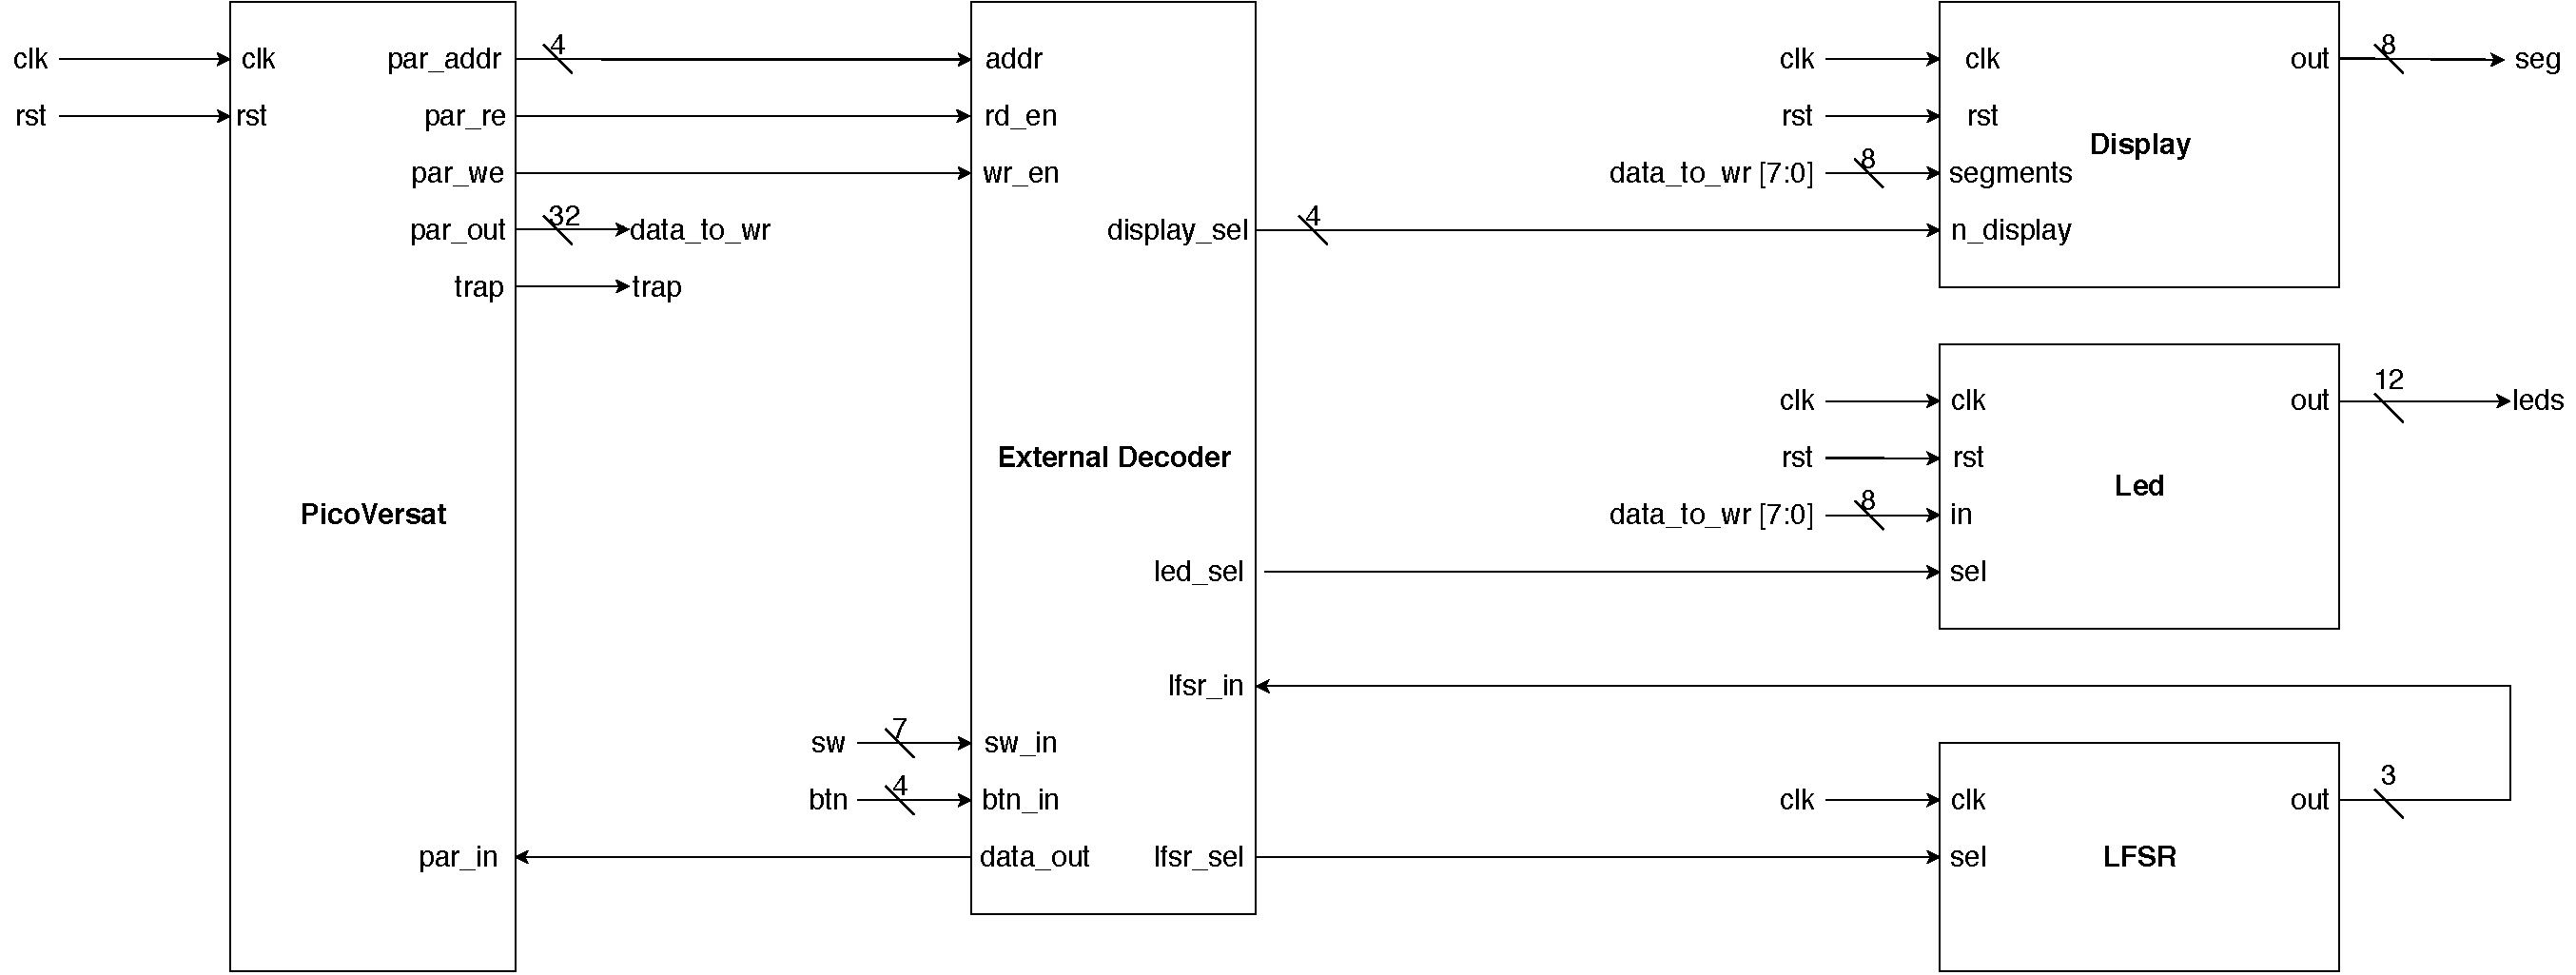
\includegraphics[scale=0.4]{ext_interface}}
    \vspace{0cm}\caption{External interface block diagram.}
    \label{fig:ext_interface}
\end{figure}

\clearpage
\subsection{Description of the display peripheral}

For each of the four digits to appear bright and continuously illuminated, all four digits should 
be driven once every 1 to 16ms. For example, for a 50 KHz clock of the FPGA, the entire display would be 
refreshed once every 16ms, and each digit would be illuminated for 1/4 of the refresh cycle, 
or 4ms. Figure~\ref{fig:temp} shows an example timing diagram for a four-digit seven-segment controller. 

\begin{figure}[!htbp]
    \centerline{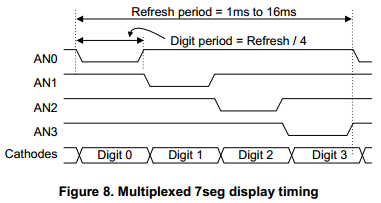
\includegraphics[scale=1.1]{temp}}
    \vspace{0cm}\caption{7 segment display timing.}
    \label{fig:temp}
\end{figure}

\vspace{10pt}
\noindent Which cathodes have to be activated to display that number. The order of the 
cathodes can be seen in figure 6 and the relation between each digit and the correspondent 
cathode code is presented in table 4. The cathode code set which of the segments of the 
display are on and off. 

\vspace{10pt}
\begin{table}[!htbp]
\centering
    \begin{tabular}{|l|l|}
    \hline
    \textbf{Content} & \textbf{Seg {[}7:0{]}} \\ \hline
    0               & 11000000               \\ \hline
    1               & 11111001               \\ \hline
    2               & 10100100               \\ \hline
    3               & 10110000               \\ \hline
    4               & 10011001               \\ \hline
    5               & 10010010               \\ \hline
    6               & 10000010               \\ \hline
    7               & 11111000               \\ \hline
    8               & 10000000               \\ \hline
    9               & 10010000               \\ \hline
    E               & 10011001               \\ \hline
    \end{tabular}
    \caption{Content available to output on displays.}
    \label{tab:disp_values}
\end{table}

\clearpage
\begin{figure}[!htbp]
    \centerline{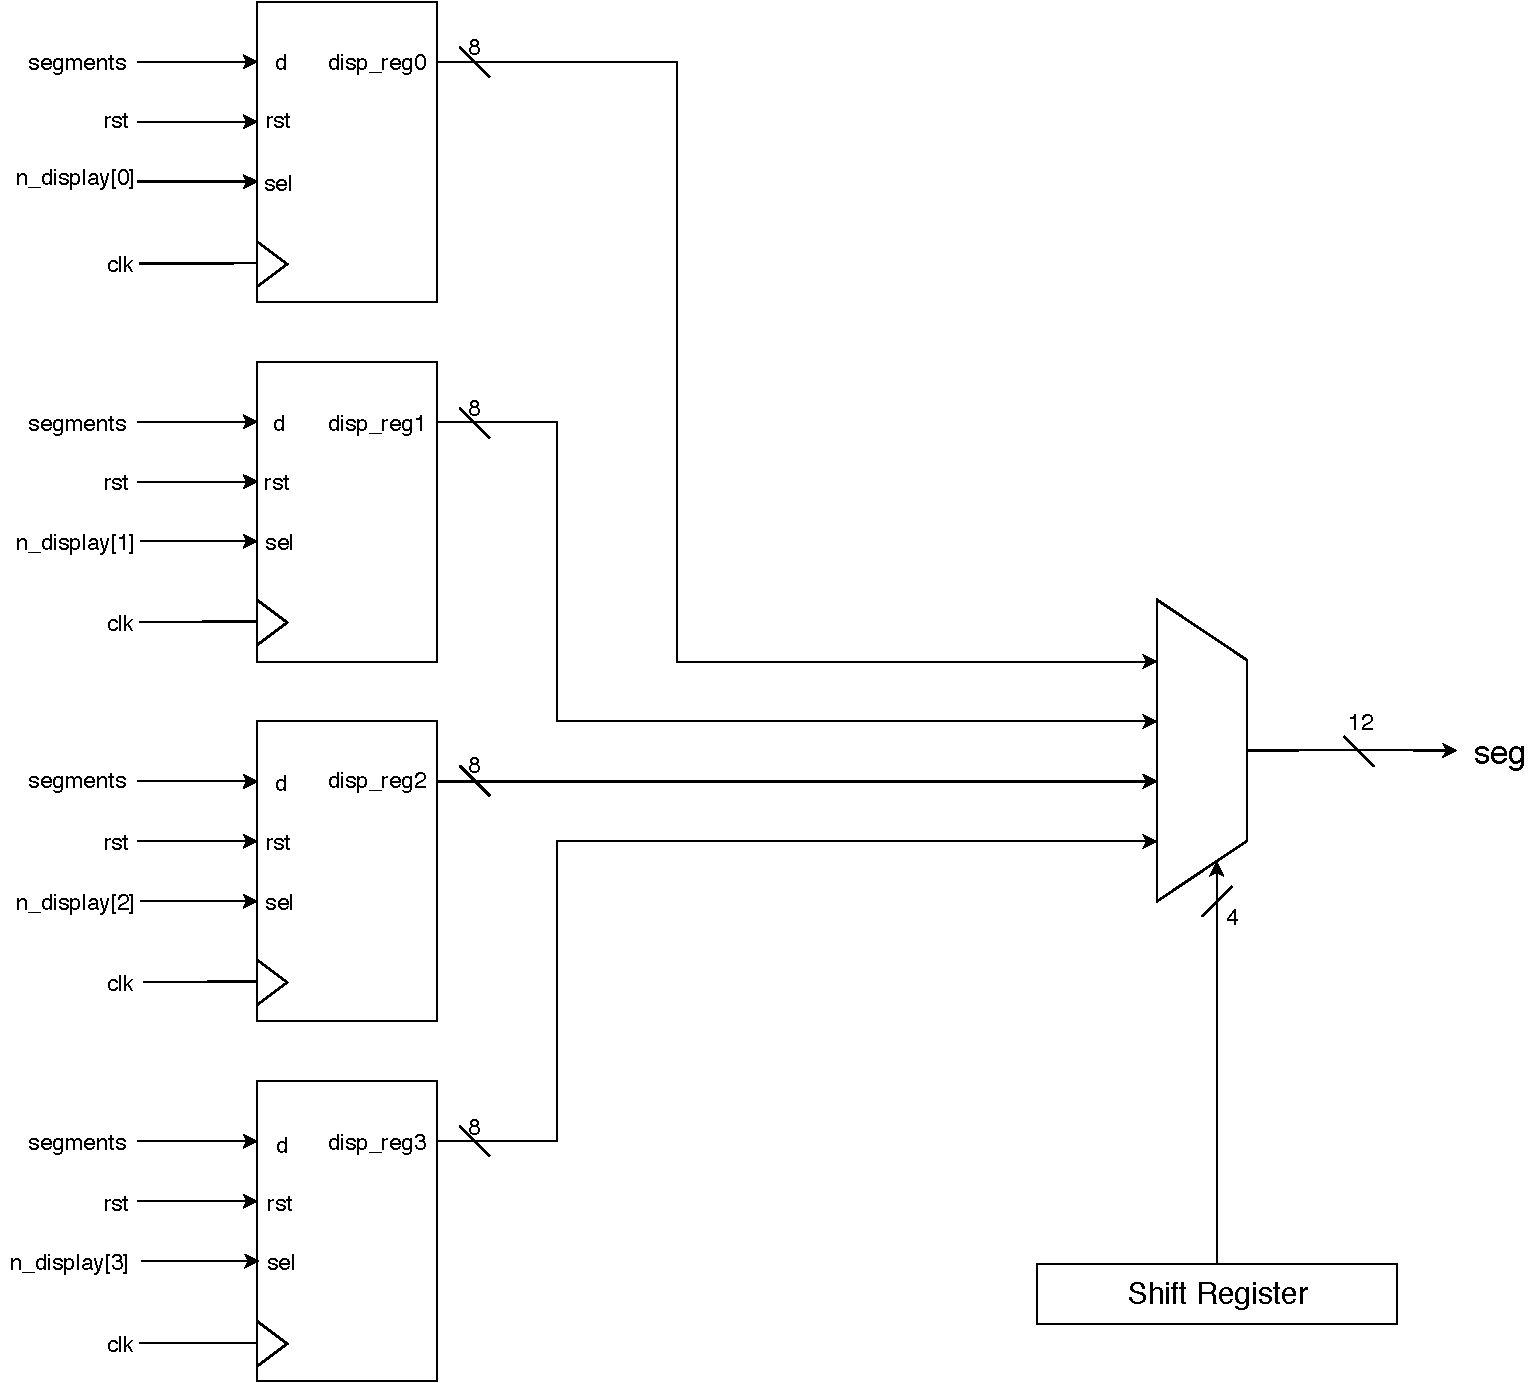
\includegraphics[scale=0.45]{display_interface}}
    \vspace{0cm}\caption{Block diagram of the display implementation.}
    \label{fig:display_interface}
\end{figure}

%\clearpage
%\subsection{Description of the buttons and switches peripheral}
%\begin{figure}[!htbp]
%    \centerline{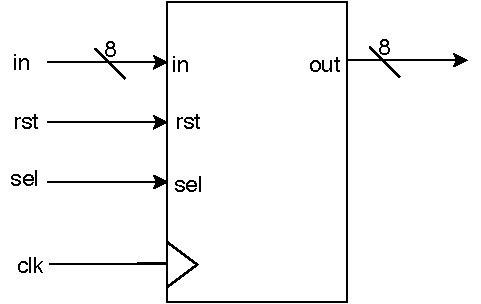
\includegraphics[scale=0.8]{switch_interface}}
%    \vspace{0cm}\caption{Buttons and switches interface.}
%    \label{fig:switch_interface}
%s\end{figure}

\clearpage
\subsection{Description of the LFSR peripheral}
Linear Feedback Shift Register (LFSR) shown in Figure~\ref{fig:LFSR}, it is a shift register 
whose input bit is a linear function of its previous state. The output from a standard shift register is fed back into its input in such a 
way as to cause the function to endlessly cycle through a sequence of patterns. Due the fact these circuit is simple to construct
and are useful on our application, it is used to generate the random sequences to the memory game.

\vspace{10pt}
\begin{figure}[!htbp]
    \centerline{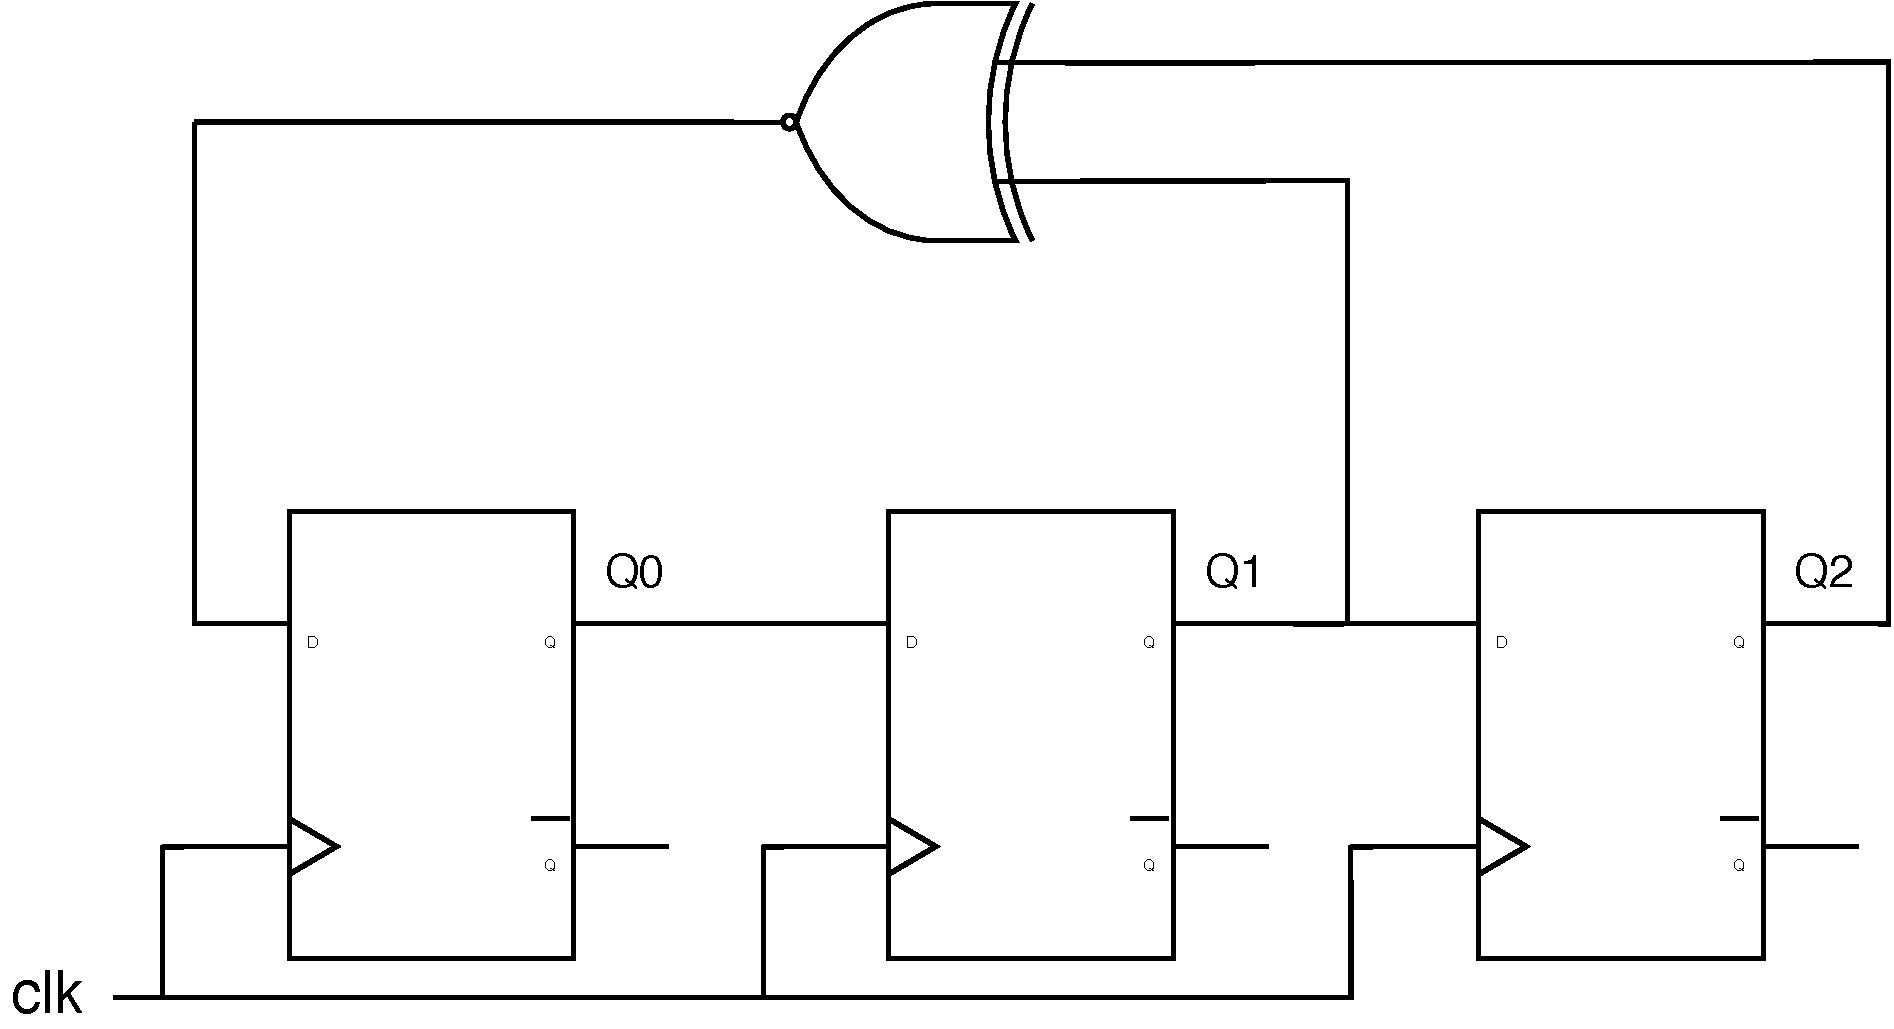
\includegraphics[scale=0.45]{LFSR}}
    \vspace{0cm}\caption{LFSR peripheral.}
    \label{fig:LFSR}
\end{figure}

\noindent The LFSR have 3 bits and the Table~\ref{tab:LFSR} shows the generation of multiple sequences contained in 
a range from [0:7]. During the development of this project we find some issues in the generation key of the game.
To resolve this problem we create a LUT with a size of 8 containing shuffled values (1,2,4,8) of the game LEDS,
finally we use the values produce by the LFSR to index this LUT to generate different sequences for the game.

\begin{table}[!htbp]
\centering
    \begin{tabular}{c|ccc}
        clk & $Q_0$ & $Q_1$ & $Q_2$ \\
        \hline
        - & 0 & 0 & 1 \\
        1 & 1 & 0 & 0 \\
        2 & 0 & 1 & 0 \\
        3 & 1 & 0 & 1 \\
        4 & 1 & 1 & 0 \\
        5 & 1 & 1 & 1 \\
        6 & 0 & 1 & 1 \\
        7 & 0 & 0 & 1 \\   
    \end{tabular}
    \caption{Truth table of the circuit LFSR.}
    \label{tab:LFSR}
\end{table} 

\clearpage
\section{Results}
\label{sec:results}

\begin{table}[!htbp]
\centering
    \begin{tabular}{|l|r|r|r|}
    \hline
    \multicolumn{4}{|c|}{\textbf{Device Utilization Summary}}                                                                                                                 \\ \hline
    \textbf{Logic Utilization}                     & \multicolumn{1}{l|}{\textbf{Used}} & \multicolumn{1}{l|}{\textbf{Available}} & \multicolumn{1}{l|}{\textbf{Utilization}} \\ \hline
    Number of Slice Flip Flops                     & 143                                & 1,920                                   & 7 \%                                      \\ \hline
    Number of 4 input LUTs                         & 901                                & 1,920                                   & 46 \%                                     \\ \hline
    Number of occupied Slices                      & 512                                & 960                                     & 53 \%                                     \\ \hline
    Number of Slices containing only related logic & 512                                & 512                                     & 100 \%                                    \\ \hline
    Number of Slices containing unrelated logic    & 0                                  & 512                                     & 0 \%                                      \\ \hline
    Total Number of 4 input LUTs                   & 929                                & 1,920                                   & 48 \%                                     \\ \hline
    Number used as logic                           & 869                                & -                                       &                                           \\ \hline
    Number used as a route-thru                    & 28                                 & -                                       &                                           \\ \hline
    Number used as 16x1 RAMs                       & 32                                 & -                                       &                                           \\ \hline
    Number of bonded IOBs                          & 34                                 & 83                                      & 40 \%                                     \\ \hline
    Number of RAMB 16s                             & 4                                  & 4                                       & 100 \%                                    \\ \hline
    Number of BUFGMUXs                             & 1                                  & 24                                      & 4 \%                                      \\ \hline
    Average Fanout of Non-Clock Nets               & 3.55                               & -                                       &                                           \\ \hline
    \end{tabular}
    \caption{Device Utilization Summary}
    \label{tab:utilization}
\end{table}

